\documentclass[a4paper,10pt]{article}
\usepackage{fontspec}
\usepackage{setspace}
\usepackage{booktabs}
\usepackage{amsmath}
\usepackage{cancel}
\usepackage{graphicx}
\usepackage{biblatex}
\usepackage{float}

\setmainfont{arial}
\setstretch{1.15}
\addbibresource{references.bib}

\title{Neural Network Concept and Implementation}
\author{Arif Suganda\\
        Tadulako University\\
        \texttt{f5522530002@untad.ac.id}
}

\begin{document}
\maketitle

\section{Manual Calculation}

Neural networks are computational models inspired by the human brain, consisting of interconnected nodes (neurons) that process information. 
Each neuron receives inputs, applies weights to them, adds a bias, and then passes the result through an activation function to produce an output.
Neural networks is calculated using the following steps:

Sum of weighted inputs and bias is calculated as follows:
\begin{equation}\label{eq:sum_weight_bias}
    z = \sum_{i=1}^{n} w_i x_i + b
\end{equation}

For this implementation we will use sigmoid activation function. Sigmoid activation function is defined as:
\begin{equation}\label{eq:sigmoid}
    \sigma(z) = \frac{1}{1 + e^{-z}}
\end{equation}

Using the output we can interpret the output as a probability of binary class and can be converted to binary output using a threshold.
The threshold can be interpreted as follows:
\begin{equation}\label{eq:threshold}
    \hat{y} = \begin{cases}
        1 & \text{if } \sigma(z) \ge 0.5 \\
        0 & \text{if } \sigma(z) < 0.5
    \end{cases}
\end{equation}

Loss function used in this implementation is Binary Cross-Entropy (BCE) which is defined as:
\begin{equation}\label{eq:bce_loss}
    L = -\left[ y \log(\hat{y}) + (1 - y) \log(1 - \hat{y}) \right]
\end{equation}

The derivative of the loss function ($L$) with respect to the sum of weighted inputs and bias (z) is calculated using the chain rule of calculus:
\begin{align}\label{eq:chain_rule}
\intertext{Chain rule application}
    \frac{\partial L}{\partial z} &= \frac{\partial L}{\partial \hat{y}} \cdot \frac{\partial \hat{y}}{\partial z} \\
\intertext{Derivative of Loss with respect to Prediction}
    \frac{\partial L}{\partial \hat{y}} &= -\left[ \frac{y}{\hat{y}} - \frac{1-y}{1-\hat{y}} \right] = \frac{\hat{y} - y}{\hat{y}(1-\hat{y})} \\
\intertext{Derivative of Prediction with respect to Sum of Weighted Inputs and Bias}
    \frac{\partial \hat{y}}{\partial z} &= \hat{y}(1 - \hat{y}) \\
\intertext{Combined Delta Calculation}
    \frac{\partial L}{\partial z} &= \frac{\hat{y} - y}{\cancel{\hat{y}(1-\hat{y})}} \cdot \cancel{\hat{y}(1 - \hat{y})} \nonumber \\
    \frac{\partial L}{\partial z} &= \hat{y} - y
\end{align}

To update the weights and bias, we use the following formulas:
\begin{align}\label{eq:update_weights_bias}
    w_i &\leftarrow w_i - \alpha \cdot \frac{\partial L}{\partial w_i} \\
    b &\leftarrow b - \alpha \cdot \frac{\partial L}{\partial b}
\end{align}

\subsection{Perceptron OR}

OR gate is a basic logic gate that outputs true (1) if at least one of the inputs is true (1). The truth table for an OR gate is as follows:
\begin{table}[h]\label{tab:or_gate}
    \centering
    \caption{Truth Table for OR Gate}
    \begin{tabular}{c c c}
        \toprule
        \textbf{Input A} & \textbf{Input B} & \textbf{Output (A + B)} \\
        \midrule
        0 & 0 & 0 \\
        0 & 1 & 1 \\
        1 & 0 & 1 \\
        1 & 1 & 1 \\
        \bottomrule
    \end{tabular}
\end{table}

A single layer perceptron is used to implement OR gate, using the code implementation provided a set of weights and bias that can be used to achieve the desired output.
The weights and bias for the OR gate can be set as follows:

\begin{figure}[H]
    \centering
    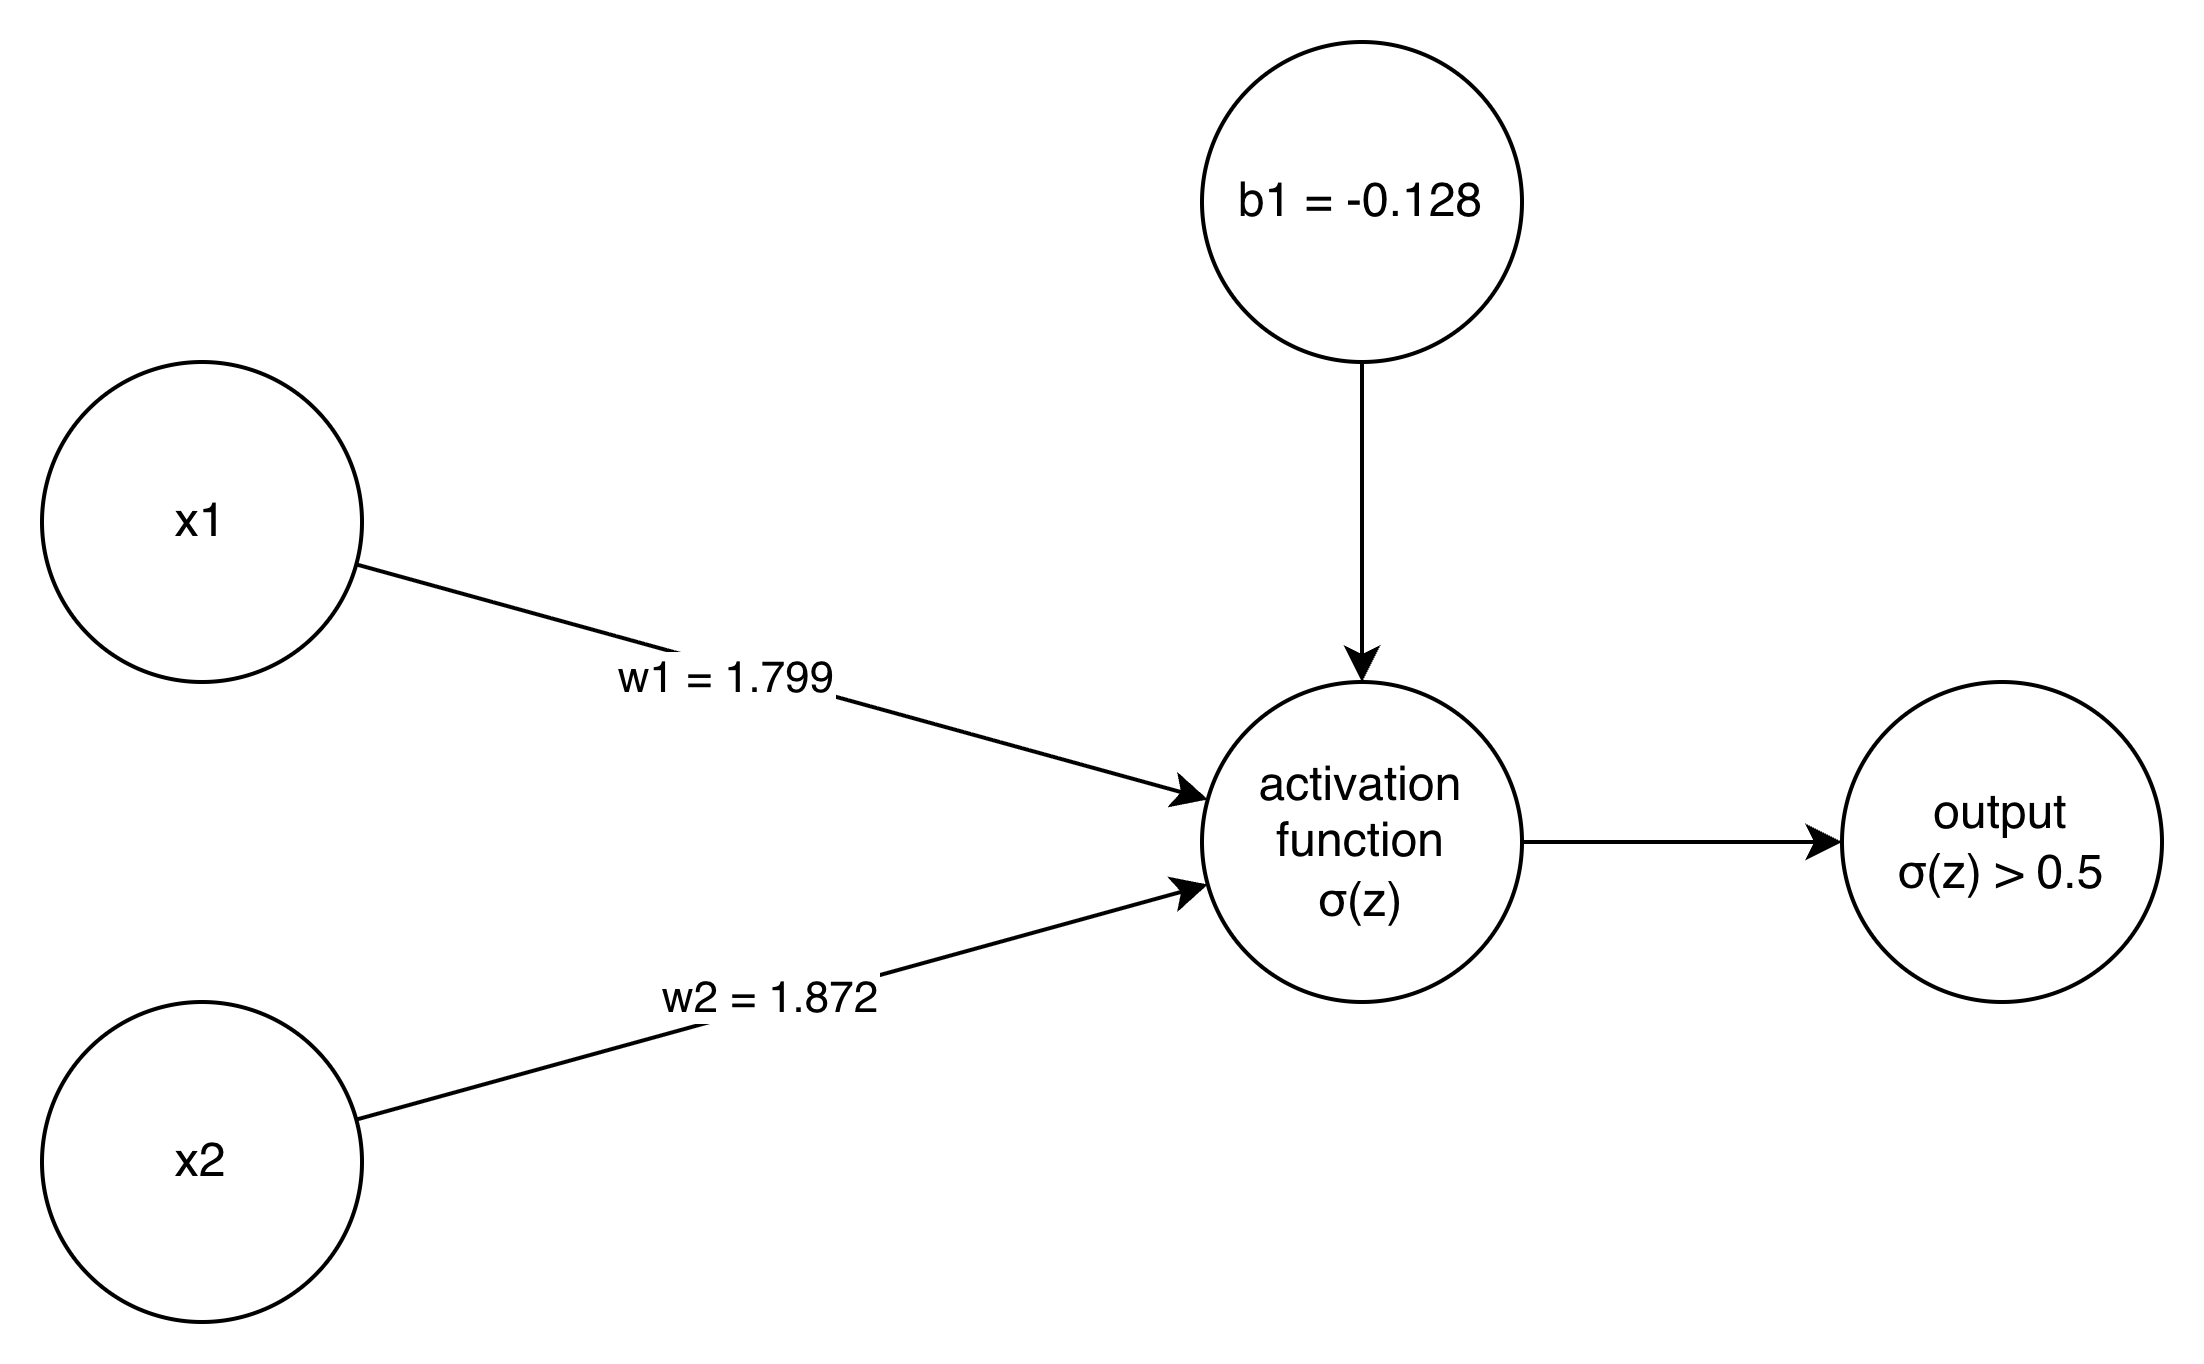
\includegraphics[width=0.8\textwidth]{perceptron_or_gate.png} 
    \caption{Diagram of a Single Layer Perceptron OR Gate}\label{fig:perceptron_or_gate}
\end{figure}

An example of the OR gate using the equation defined the previous section is perform as follows:
\begin{align*}
    z &= w_1 x_1 + w_2 x_2 + b \\
    z &= 1.799 * 0 + 1.872 * 1 + -0.128 \\
    z &= 0 + 1.872 -0.128 \\
    z &= 1.744 \\
    \hat{y} &= \sigma(z) = \frac{1}{1 + e^{-1.744}} \\
    \hat{y} &= 0.846 \\
    \hat{y} &= \begin{cases}
        1 & \text{if } \sigma(z) \ge 0.5 \\
        0 & \text{if } \sigma(z) < 0.5
    \end{cases}\\
    \hat{y} &= 1
\end{align*}

\subsection{Perceptron XOR}

XOR gate is a basic logic gate that outputs true (1) if exactly one of the inputs is true (1). The truth table for an XOR gate is as follows:
\begin{table}[h]
    \centering
    \caption{Truth Table for XOR Gate}\label{tab:xor_gate}
    \begin{tabular}{c c c}
        \toprule
        \textbf{Input A} & \textbf{Input B} & \textbf{Output (A + B)} \\
        \midrule
        0 & 0 & 0 \\
        0 & 1 & 1 \\
        1 & 0 & 1 \\
        1 & 1 & 0 \\
        \bottomrule
    \end{tabular}
\end{table}

Multi layer perceptron is used to implement XOR gate, using the code implementation provided a set of weights and bias that can be used to achieve the desired output.
The weights and bias for the XOR gate can be set as follows:

\begin{figure}[H]
    \centering
    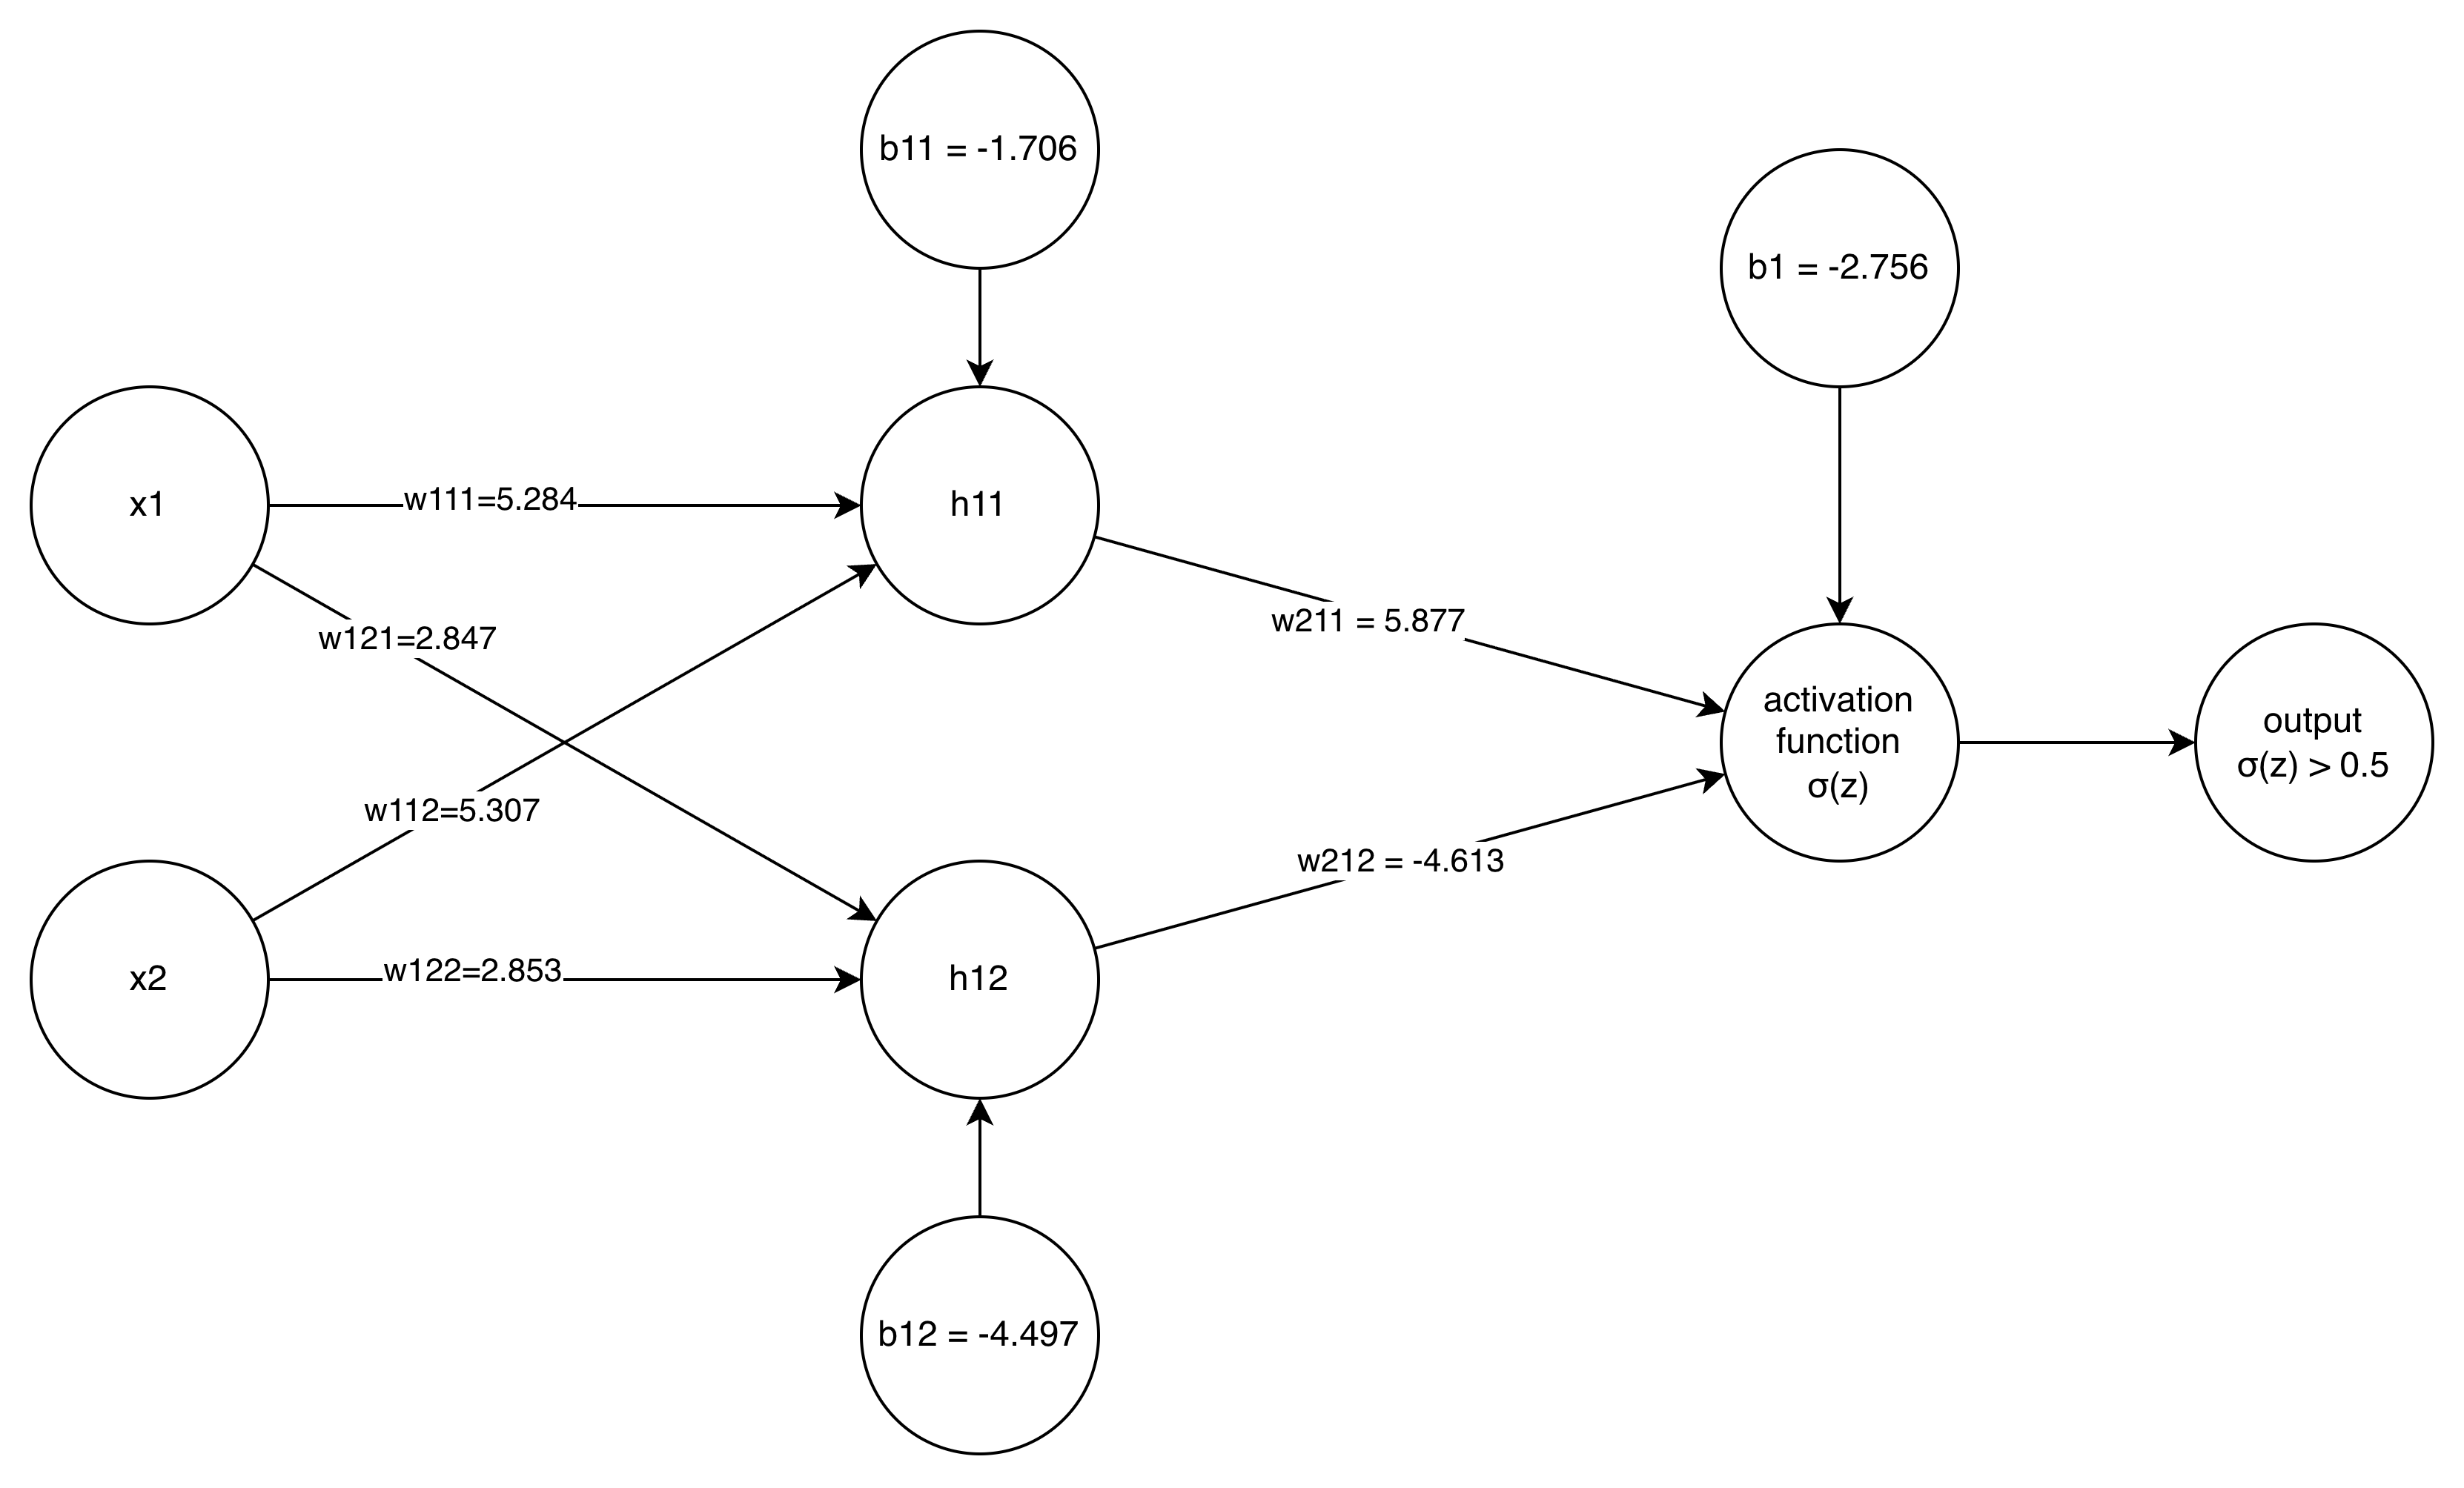
\includegraphics[width=1\textwidth]{perceptron_xor_gate.png} 
    \caption{Diagram of a Single Layer Perceptron XOR Gate}\label{fig:perceptron_xor_gate}
\end{figure}

An example of the XOR gate using the equation defined the previous section is perform as follows:
\begin{align*}
\intertext{$\sigma_{11}$ calculation}
    z_{11} &= w_{111} x_1 + w_{112} x_2 + b \\
    z_{11} &= 5.284 * 0 + 5.307 * 1 + (-1.706) \\
    z_{11} &= 0 + 5.307 - 1.706 \\
    z_{11} &= 3.601 \\
    \sigma(z_{11}) &= \sigma(z_{11}) = \frac{1}{1 + e^{-3.601}} \\
    \sigma(z_{11}) &= 0.974 \\
\intertext{$\sigma_{12}$ calculation}
    z_{12} &= w_{121} x_1 + w_{122} x_2 + b \\
    z_{12} &= 2.847 * 0 + 2.853 * 1 + (-4.497) \\
    z_{12} &= 0 + 2.853 - 4.497 \\
    z_{12} &= -1.644 \\
    \sigma(z_{12}) &= \sigma(z_{12}) = \frac{1}{1 + e^{-(-1.644)}} \\
    \sigma(z_{12}) &= 0.838 \\
\intertext{$\hat{y}$ calculation}
    z_{21} &= w_{211} x_1 + w_{212} x_2 + b \\
    z_{21} &= 5.877 * 0.974 + (-4.613) * 0.838 + (-2.756) \\
    z_{21} &= 5.724 - 3.865 - 2.756 \\
    z_{21} &= -0.897 \\
    \hat{y} &= \sigma(z_{21}) = \frac{1}{1 + e^{-(-0.897)}} \\
    \hat{y} &= 0.710 \\
    \hat{y} &= \begin{cases}
        1 & \text{if } \sigma(z) \ge 0.5 \\
        0 & \text{if } \sigma(z) < 0.5
    \end{cases}\\
    \hat{y} &= 1
\end{align*}

\subsection{Implementation XOR} \label{sec:implementation_xor}

Implementation of XOR gate using multi-layer perceptron is performed using architecutre as shown in figure~\ref{fig:perceptron_xor_gate}.
The implementation is performed using python and numpy library, the code implementation for sigmoid, derivative of sigmoid, sum of weighted inputs and bias, loss function, and delta calculation is as follows:
\begin{verbatim}
def sigmoid(x):
    return 1 / (1 + np.exp(-x))

def sigmoid_derivative(x):
    return x * (1 - x)

def calculate_layer(inputs, weights, bias):
    sum_ = np.dot(inputs, weights)
    sum_bias = sum_ + bias
    return sum_bias, sigmoid(sum_bias)

def calculate_loss(y_true, y_pred):
    y_pred_clipped = np.clip(y_pred, 1e-15, 1 - 1e-15)
    return -np.mean(
        y_true * np.log(y_pred_clipped) + 
        (1 - y_true) * np.log(1 - y_pred_clipped)
    )

def calculate_delta(y_true, y_pred):
    return  y_pred - y_true

\end{verbatim}

The training process is performed using backpropagation algorithm, the code implementation for training the model is as follows:
\begin{verbatim}
def train(X, y, layers, epochs=200, lr=1):
    n_layers = len(layers)
    i_bias = 1
    i_weight = 0
    histories = []
    
    for i in range(epochs):
        # Forward
        current_input = X
        layers_output = [X]
        
        for layer in layers:
            _, current_input = calculate_layer(
                current_input, 
                layer[i_weight], 
                layer[i_bias]
            )
            layers_output.append(current_input)

        # Backpropagation
        d_layers_output = []
        
        # Loss function and output layer delta
        delta = calculate_delta(y, layers_output[-1])
        d_layers_output.append(delta)
        
        # Hidden layer propagation
        for j in range(n_layers - 1, 0, -1):
            weight = delta.dot(layers[j][i_weight].T)
            delta = weight * sigmoid_derivative(
                layers_output[j])
            d_layers_output.append(delta)
        d_layers_output.reverse()
        
        # Update weight
        for j in range(n_layers):
            layer_input = layers_output[j]
            delta_j = d_layers_output[j]
            
            layers[j][i_weight] -= layer_input.T.dot(
                delta_j) * lr
            layers[j][i_bias] -= np.sum(
                delta_j, axis=0, keepdims=True) * lr
        
        histories.append([[
            w.copy(), b.copy()] for w, b in layers ])
        
    return histories, layers

\end{verbatim}

The training process is done for 200 epochs with a learning rate of 1, the initialization of weights and bias is performed using random values, and the code implementation for initialization is as follows:
\begin{verbatim}
n_input_neurons = 2
n_hidden_neurons = 2
n_output_neurons = 1

layers = []

w_hidden = np.random.uniform(
    size=(n_input_neurons, n_hidden_neurons))
b_hidden = np.zeros((1, n_hidden_neurons))
layers.append([w_hidden, b_hidden])

w_out = np.random.uniform(
    size=(n_hidden_neurons, n_output_neurons))
b_out = np.zeros((1, n_output_neurons))
layers.append([w_out, b_out])

# # XOR
X = np.array([[0,0], [0,1], [1,0], [1,1]])
y = np.array([[0], [1], [1], [0]])

histories, model = train(X, y, layers)

\end{verbatim}

The result of this implementation can be seen in figure~\ref{fig:xor_gate_implementation} which shows the output of the model after training, where the output is close to the expected output of the XOR gate.

\begin{figure}[H]
    \centering
    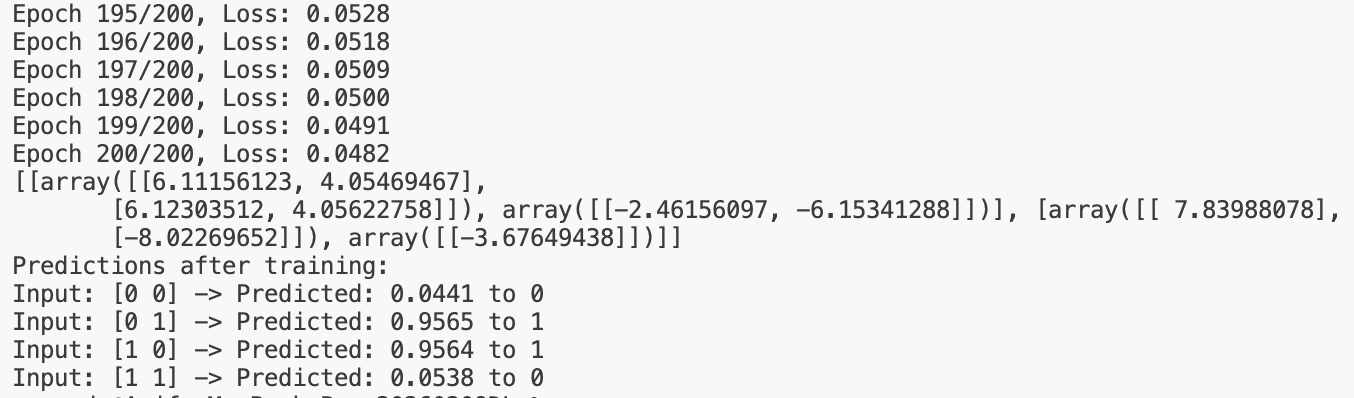
\includegraphics[width=1\textwidth]{xor_gate_implementation.png} 
    \caption{XOR Gate Implementation Result}\label{fig:xor_gate_implementation}
\end{figure}

\section{Architecture and Function}

The explanation of the architecture and function of the neural network is using the implementation of the XOR gate as shown in figure~\ref{fig:xor_architecture}.
\begin{figure}[H]
    \centering
    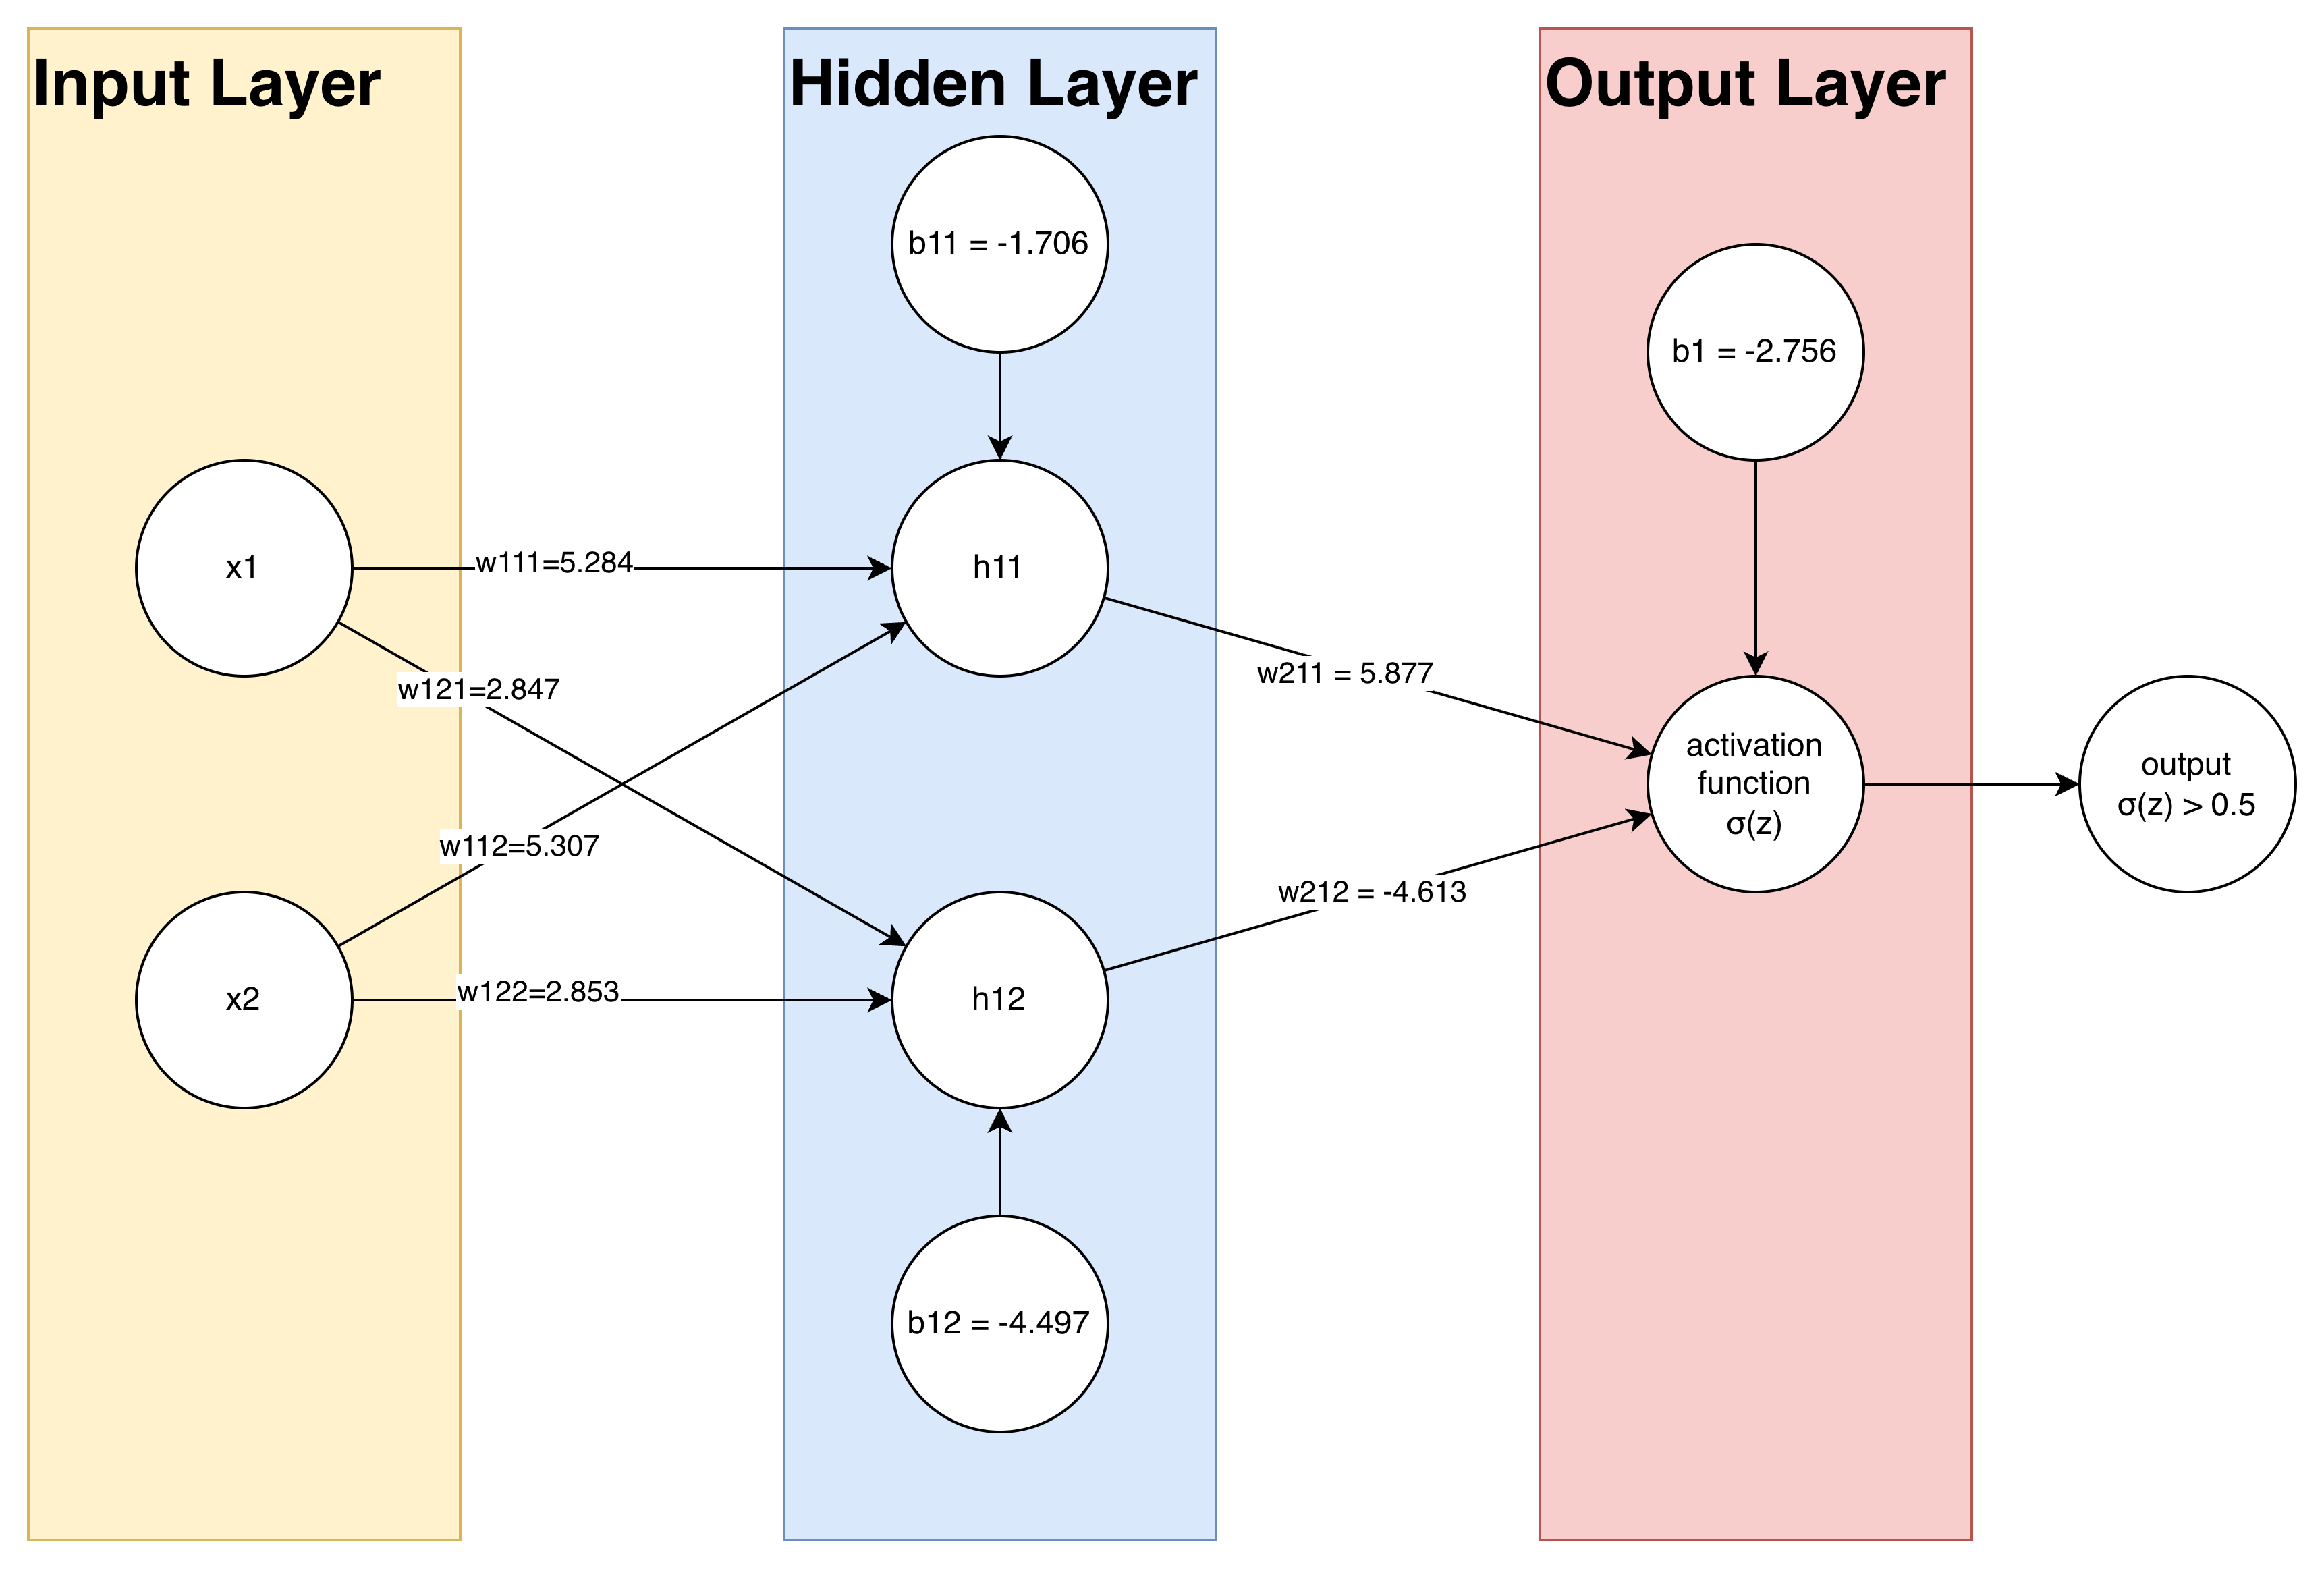
\includegraphics[width=1\textwidth]{xor_architecture.png} 
    \caption{XOR Gate Architecture}\label{fig:xor_architecture}
\end{figure}

\subsection{Structure}
The architecture of the neural network used in this implementation is a multi-layer perceptron with one hidden layer, where the input layer consists of 2 neurons, the hidden layer consists of 2 neurons, and the output layer consists of 1 neuron.
Each neuron connects to the next layer with a set of weights and bias, where the weights determine the strength of the connection between neurons and bias detemines the threshold for activation.
The weights and bias are then updated during the training process using backpropagation to better shift the output towards the expected output by minimizing the loss function.

\subsection{Layers role and data flow}
\begin{enumerate}
    \item Input Layer: The input layers consists of 2 neurons representing the two inputs of the XOR gate.
    The input layer does not perform any computations, it simply passes the input data to the next layer.
    \item Hidden Layer: The hidden layer consists of 2 neurons that receive the input from the input layer, calculate the sum of the weighted inputs and bias, apply the activation function, and pass the output to the next layer.
    The hidden layer allows the model to learn the non-linear relationship between the inputs and output of the XOR gate.
    \item Output Layer: The output layer consists of 1 neuron that receives the input from the hidden layer, calculates the sum of the weighted inputs and bias, applies the activation function, and produces the final output of the model which determines the prediction of the XOR gate.
\end{enumerate}

\subsection{Dimension, neurons, and model complexity}
The architecture of the neural network implemented in this example has a total of 5 neurons and 9 parameters (weights and bias).
The number of neurons and parameters in this model is sufficient to learn the XOR gate, which is a non-linear problem that cannot be solved by a single layer perceptron.
The complexity of this model is extremely low compared to more complex neural network achitectures used in the real world applications.
The architecture of this model can be an example of how a simple multi-layer perceptron can be used to solve a non-linear problem, and it serves as a foundation for understanding more complex neural network architectures.

\subsection{Example}
An example of how neural network is used in the real world application can be seen in the many field such as image recognition, natural language processing, speech recognition, generative modeling, and many more.
A simple example of neural network can be seen in the Section~\ref{sec:implementation_xor} where a multi-layer perceptron is used to implement the XOR gate, which is a binary classification problem that can be solved using a simple neural network architecture.

\section{Mathematical Detail of Neural Networks}

The Neural network works using a series of mathematical operation based of the input data.
The neuron of the network performs a sum of weighted inputs and bias (eq~\ref{eq:sum_weight_bias}), appy their activation function (eq~\ref{eq:sigmoid}), and pass its output to the next layer.
The result of these operations is a prediction output that can be used to find the loss function (eq~\ref{eq:bce_loss}), which measures the difference between the predicted output and the true output.
The loss function is then used to calculate the delta (eq~\ref{eq:chain_rule}), which determines how much the weights and bias should be updated during the training process(eq~\ref{eq:update_weights_bias}).

The adjustment of weights and bias is calculated using backpropagation algorithm, using the chain rule of calculus to propagate the error of the prediction to each neuron within the network, then use the error to update their own weight and bias.
These update will minimize the loss function, allowing the model to fit the data, learn from it and improve its performance over time.

The chain rule of calculus using sigmoid and binary cross-entropy can be seen in the equation~\ref{eq:chain_rule} where the rate of change is $\frac{\partial L}{\partial z} = \hat{y} - y$.
These chain of mathematical operation ensure that the model does not just update the weights and bias randomly, but using its own data and the error calculated from the loss function.

The usage of loss function and backpropagation algorithm allows the model to learn from its own mistakes by ensuring the changes in the network are grounded on data and error from its own prediction, and ultimately learn from it.

\end{document}